\subsubsection{Shadow DOM}
\label{sec:3_WC_Shadow_DOM}

Mit Hilfe von Shadow DOM können Elemente mit einer neuen Art von Knoten verbunden werden. Diese neue Art von Knoten wird auch \glqq Shadow Root\grqq\ genannt. Ein Element, dass einer Shadow-Root zugeordnet ist, wird auch als \glqq Shadow-Host\grqq\ bezeichnet. Anstatt den Inhalt eines Shadow-Hosts zu rendern, wird der des Shadow-Root gerendered.

\begin{lstlisting}[language=HTML, caption={Shadow-Root Beispiel eines Buttons}, label={lst:3_ShadowDomBasic1}, escapeinside={@}{@}]
<button>Hello, world!</button>
<script>
  var host = document.querySelector('button');
  var root = host.createShadowRoot();
  root.textContent = '@\begin{CJK}{UTF8}{bsmi}@こんにちは、影の世界@\end{CJK}@!';
</script>
\end{lstlisting}

Code-Beispiel \ref{lst:3_ShadowDomBasic1} rendert zuerst das in Abbildung \ref{sfig:3_ShadowDom1} auf Seite \pageref{sfig:3_ShadowDom1} gezeigte Ergebnis. Danach wird mit Hilfe von JavaScript und ShadowDOM das Element, wie in Abbildung \ref{sfig:3_ShadowDom2} auf Seite \pageref{sfig:3_ShadowDom2} zu sehen ist, verändert.

\begin{figure}[h]
  \centering
  \subfloat[HTML gerendertes Element]{
    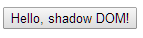
\includegraphics[]{images/SS1.png}
    \label{sfig:3_ShadowDom1}
  }
  \qquad
  \subfloat[HTML Element mit Hilfe von JavaScript und Shadow DOM manipuliert]{
    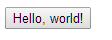
\includegraphics[]{images/SS2.png}
    \label{sfig:3_ShadowDom2}
  }
  \caption[
    Beispiel einer Shadow-Root Node
  ]{
    Beispiel einer Shadow-Root Node
  }
  \label{sfig:3_ShadowDom}
\end{figure}

Darüber hinaus wird das Resultat, wenn man den \lstinline|<button>| nach seinem Inhalt mit Hilfe der \lstinline|textConten| Eigenschaft abfragt nicht
\begin{lstlisting}[escapeinside={@}{@}]
@\begin{CJK}{UTF8}{bsmi}@こんにちは、影の世界@\end{CJK}@!'
\end{lstlisting}
zurückgegeben, sondern \lstinline|"Hello, world!"|, weil die DOM-Unterstruktur unter der Shadow-Root vollständig gekapselt ist.

Es ist zu erwähnen, dass dies ein sehr schlechtes Beispiel ist, da sämtlicher Inhalt im Shadow-DOM nicht für Suchmaschinen, Erweiterungen, Screen readers, etc. erreichbar ist. Shadow-DOM ist nur für sematisch bedeutungsloses Markup, das benötigt wird um eine Webkomponente zu erstellen.

\textbf{Trennung von Inhalt und Darstellung}

Code-Beispiel \ref{lst:3_ShadowDomBasic2} auf Seite \pageref{lst:3_ShadowDomBasic2} wird als Ausgangsbasis dieses Beispiels genommen. Abbildung \ref{fig:3_ShadowDom2} auf Seite \pageref{fig:3_ShadowDom2} zeigt diese Grundbasis, um mit darauffolgenden Schritten sämtlichen Inhalt von der Darstellung zu trennen.

\begin{lstlisting}[language=HTML, caption={Namensschild ohne Shadow-DOM - Ausgangsbasis um Inhalt von Darstellung zu trennen}, label={lst:3_ShadowDomBasic2}, escapeinside={@}{@}]
<style>
.outer {
  border: 2px solid brown;
  border-radius: 1em;
  background: red;
  font-size: 20pt;
  width: 12em;
  height: 7em;
  text-align: center;
}
.boilerplate {
  color: white;
  font-family: sans-serif;
  padding: 0.5em;
}
.name {
  color: black;
  background: white;
  font-family: "Marker Felt", cursive;
  font-size: 45pt;
  padding-top: 0.2em;
}
</style>
<div class="outer">
  <div class="boilerplate">
    Hi! My name is
  </div>
  <div class="name">
    Bob
  </div>
</div>
\end{lstlisting}

\begin{figure}[h]
\centering
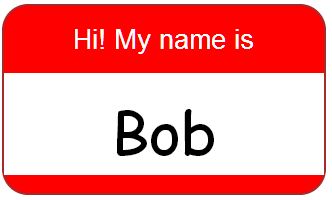
\includegraphics[height=5.0cm]{images/SS3.png}
\caption[
  Ausgangsbeispiel von der Trennung von Darstellung und Inhalt bei Shadow-DOM
]{Ausgangsbeispiel von der Trennung von Darstellung und Inhalt bei Shadow-DOM}
\label{fig:3_ShadowDom2}
\end{figure}

Dadurch, dass dem DOM-Baum Kapselung fehlt, ist die gesamte Struktur des Namensschildes im Dokument sichtbar. Wenn beispielsweise andere Elemente auf der Webseite dieselben Klassennamen verwenden würden, würde das Aussehen von dem nicht zum gewünschten Ergebnis führen.

\begin{enumerate}
\litem{Verstecken von Darstellungsdetails} \hfill \\
Semantisch gibt es nur zwei wichtige Informationen bei diesem Beispiel:
\begin{enumerate}
\item Es handelt sich um ein Namensschild
\item Der Name ist \glqq Bob\grqq .
\end{enumerate}
Daraus wird das Markup erstellt, das semantisch näher bei der gewünschten Information ist.

\begin{lstlisting}[language=HTML, caption={Darstellung des Markups mit der gewünschten Information ohne Darstellung}, label={lst:3_ShadowDomBasic3}, escapeinside={@}{@}]
<div id="nameTag">Bob</div>
\end{lstlisting}

Des Weiteren wird sämtlicher Code, der der Darstellung dient, in ein \lstinline|<template>|-Element gepackt.

\begin{lstlisting}[language=HTML, caption={Darstellung des Markups mit der gewünschten Information mit Hilfe von einem Template}, label={lst:3_ShadowDomBasic4}, escapeinside={@}{@}]
<div id="nameTag">Bob</div>
<template id="nameTagTemplate">
<style>
.outer {
  border: 2px solid brown;
  border-radius: 1em;
  background: red;
  font-size: 20pt;
  width: 12em;
  height: 7em;
  text-align: center;
}
.boilerplate {
  color: white;
  font-family: sans-serif;
  padding: 0.5em;
}
.name {
  color: black;
  background: white;
  font-family: "Marker Felt", cursive;
  font-size: 45pt;
  padding-top: 0.2em;
}
</style>
<div class="outer">
  <div class="boilerplate">
    Hi! My name is
  </div>
  <div class="name">
    Bob
  </div>
</div>
</template>
\end{lstlisting}

Zu diesem Zeitpunkt wird \glqq Bob\grqq\ das einzige sein, das gerendered wird. Da sämtliche Code, der der Darstellung dient, in ein \lstinline|<template>| gepackt wurde, muss man dies beispielsweise mit JavaScript hinzufügen. In Code-Beispiel \ref{lst:3_ShadowDomBasic5} auf Seite \pageref{lst:3_ShadowDomBasic5} wird zuerst eine Shadow-Root am Element \lstinline|<div id=nameTag></div>| erstellt. Danach wird nach dem Template gesucht und der Inhalt an die Shadow-Root angefügt.

\begin{lstlisting}[language=JavaScript, caption={Hinzufügen des Inhalts eines Templates in eine Shadow-Root}, label={lst:3_ShadowDomBasic5}, escapeinside={@}{@}]
<script>
  var shadow = document.querySelector('#nameTag').createShadowRoot();
  var template = document.querySelector('#nameTagTemplate');
  shadow.appendChild(template.content);
</script>
\end{lstlisting}

Da man nun eine Shadow-Root gesetzt und mit Markup versehen hat wird das Namensschild wieder gerendert. Wenn das Element inspiziert wird, sieht man nur die gewünschte Information, ohne Darstellungselementen.

Dies zeigt, dass durch die Verwendung von Shadow-DOM sämtliche Darstellungendetails im Shadow-DOM gekapselt wurden und von außen nicht erreichbar sind.

\litem{Trennung von Inhalt und Darstellung} \hfill \\
Mit Hilfe von Code-Beispiel \ref{lst:3_ShadowDomBasic4} und \ref{lst:3_ShadowDomBasic5} werden sämtliche Darstellungsdetails versteckt, jedoch wurde der Inhalt noch nicht mit der Darstellung getrennt. Wenn man beispielsweise den Namen des Namensschildes austauschen müsste, müsste man es an zwei Stellen machen. Einerseits an der Stelle im Template und andererseits an der Stelle des \lstinline|<div id=nameTag></div>|-Elements.

Um den tatsächlichen Inhalt von sämtlichen Darstellungen zu trennen, muss eine Komposition von Elementen benutzt werden. Das Namensschild setzt sich einerseits aus dem roten Hintergrund mit den \glqq Hi! My name is\grqq -Text zusammen und andererseits dem Namen der Person.

Als Autor einer Komponente entscheidet man, wie die Komposition des erstellten Elements funktionieren soll, mit Hilfe des \lstinline|<content>|-Elements. Dieses Element erstellt einen Einsatzpunkt in der Darstellung und sucht Inhalte aus dem Shadow-Host, die an dieser Stelle dargestellt werden sollten.

\begin{lstlisting}[language=HTML, caption={Erweiterung des Code-Beispiels \ref{lst:3_ShadowDomBasic4} mit dem <content>-Element}, label={lst:3_ShadowDomBasic6}, escapeinside={@}{@}]
<div id="nameTag">Bob</div>
<template id="nameTagTemplate">
<style>
.outer {
  border: 2px solid brown;
  border-radius: 1em;
  background: red;
  font-size: 20pt;
  width: 12em;
  height: 7em;
  text-align: center;
}
.boilerplate {
  color: white;
  font-family: sans-serif;
  padding: 0.5em;
}
.name {
  color: black;
  background: white;
  font-family: "Marker Felt", cursive;
  font-size: 45pt;
  padding-top: 0.2em;
}
</style>
<div class="outer">
  <div class="boilerplate">
    Hi! My name is
  </div>
  <div class="name">
    <content></content>
  </div>
</div>
</template>
\end{lstlisting}

In Code-Beispiel \ref{lst:3_ShadowDomBasic6} auf Seite \pageref{lst:3_ShadowDomBasic6} wird das Namensschild mit dem vom Shadow-Host projizierten Inhalt in das \lstinline|<content>|-Element gerendered.
Dies vereinfacht die Struktur des Dokuments, da der Name nur noch an einer Stelle vorhanden ist. Wenn man nun den Namen aktualisieren möchte, kann man das mit folgender Methode tun: \lstinline|document.querySelector('#nameTag').textContent = 'Shellie';|.

Das Namensschild wird automatisch nach Zuweisung eines neuen Namens aktualisiert, da der Inhalt vom Namensschild in das \lstinline|<content>|-Element projiziert wird. Somit wurde die Trennung von Inhalt und Darstellung erreicht.
\end{enumerate}